\section{Photons}

\begin{enumerate}
    
    \item
	Directly ionizing radiation: Fast particles having a charge that transfers energy through a series of small Coulomb interactions.
    \item
	Indirectly ionizing radiation: Photons or neutrons which transfer energy to charged particles in the matter.

\end{enumerate}

The "cross section" is proportinonal with the interaction strenght.
A simple visulisation could be imagining two disks of radiis $r$, the total area is then 

\begin{equation}
    s = \pi (r_1^2 + r_2^2)
\end{equation}

Consider now $N$ particles coming towards an area $S$ with $n$ atoms.
The probability for interaction then becomes 

\begin{equation}
    p = \frac{n*\sigma}{S}
\end{equation}

and the with the number of \emph{interacting} particles

\begin{equation}
    Np = N\frac{n*\sigma}{S}
\end{equation}

We separate between electronic and atomic cross sections.
The cross sections depends on the type of target, and the type of the incoming particle.

The differential cross section is the number of particles scattered into the angle d$\Omega$ per units area.
For photons we can have (in principle) two different kinds of processes:

\begin{enumerate}

    \item
	Absorbtion
    \item
	Scattering
\end{enumerate}

\subsection{Scattering, Thompsom and Comton}

The scattering can be coherent, or incoherent. 

The coherent scattering is called Rayleigh scattering. Here the photon is scattered without loss of energy

The atomic cross section for Rayleigh-scattering is 

\begin{equation}
    \sigma_r \propto \left( \frac{Z}{h\upsilon} \right)^2
\end{equation}

Dependence mainly on atomic structire and photon energy. 
Larger $Z$ and smaller $h\upsilon$ will increase the chance for Rayleigh scattering

The incoherent scattering is called Comtpon-scattering.
Here, the photon will hit an electron (which can be considered almost free) and loose some energy.

We can simply consider the kinematics of what is happening and get the result:

\begin{equation}
    h\upsilon = \frac{h\upsilon}{1 + \frac{h\upsilon}{m_e c^2}(1 - \mathrm{cos} \theta)}
\end{equation}

The forward-scattered photons will have the same energy as the incoming photons, whereas the scattered photons of other angles will have lower and lower energy.
The cross section of Compton-scattering was derived by Klein and Nishina, with a free electron assumed

\begin{equation}
    \left( \frac{\mathrm{d}\sigma}{\mathrm{d}\theta} \right ) = \pi r_0^2 \left( \frac{\upsilon'}{\upsilon} \right)^2 \left( \frac{\upsilon'}{\upsilon} + \frac{\upsilon}{\upsilon'} - \mathrm{sin}^2\theta \right ) \mathrm{sin} \theta
\end{equation}

We can perform some substitution to get the cross section for a certain scatter-energy 

\begin{equation}
    \frac{\mathrm{d}\sigma}{\mathrm{d} ( h\upsilon')} = \frac{\pi r_0^2 m_e c^2}{(h \upsilon)^2} \left ( \frac{h\upsilon'}{h\upsilon} + \frac{h\upsilon}{h\upsilon'} -1 + \left ( 1  - \left( \frac{h\upsilon}{h\upsilon'} -1 \right ) \frac{m_e c^2}{h\upsilon} \right ) ^2 \right )
\end{equation}

The fractional cross section with respect to the scattered energy has a sharp rise at the lower limit, this is because the back-scattered photons can only have a certain energy.
At the upper max we could have a compton-edge, a rise of the cross section before an abrupt stop while we approach the incoming energy.

%\begin{figure}
%    \centering
%    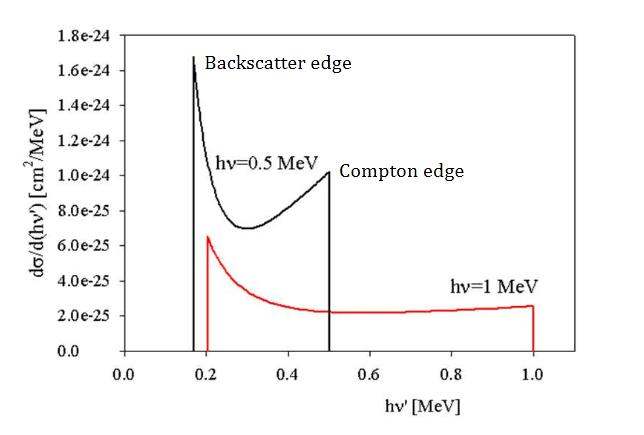
\includegraphics[width = 0.48\textwidth]{photons/figs/kleinnishinaenergy}
%    \caption{Fractional cross section as a function of energy of the scattered photon}
%\end{figure}

The Klein-Nishina cross section assumes a "free" electron, and for atomic electrons and for lower photon energies, this do not hold.
The cross section then becomes smaller for high $Z$-materials for lower energies.

In the compton process, some energy gets transfered to the electron:

\begin{equation}
    T = h\upsilon - h \upsilon'
\end{equation}

This energy transfer can be expressed as a fractional cross section, and gives a nice expression for the mean transfered energy

\begin{equation}
    \bar{T} = \frac{\sigma_{tr}}{\sigma} h \upsilon
\end{equation}

\subsection{Photo-electric effect}

A photon is absorbed by an atom or molecule, it can result in an excitation or an ionization.
An electron is ejected from the atom.
When the atom de-excites, it can give off characteristic radiation.

